\chapter{Parallel Computation: N-Loop, N-Order systems (N-OS)\index{N-OS: Nth order system -- cellular system}}\label{lect6b}
\localtoc

As we saw in the second part of this book, we were able to achieve the requirements of a computing system by successively introducing feedback loops starting from combinational circuits, circuits without loops. Can we continue the process of closing new loops? Could we have an additional gain from these additional loops? We will try to answer these questions in the following.

\section{Cellular Automata (CA)\index{CA (cellular automaton)!theoretical infinite CA}}

Each new loop increases, as we have seen in the previous chapters, the complexity and the autonomy of the system. When the number of loops is $N$, for any large $N$, we cannot keep the increase in complexity at a level that corresponds to the number of loops. For this, the loops must close over identical systems to keep the complexity independent of $N$. Thus, even once the size becomes proportional to $N$, the complexity (the size of the shortest description) remains independent of $N$ and we can afford to keep the complexity independent of size. Moore's law ensures exponential growth only for size, but not for complexity. In other words, we can exponentially increase the size of the hardware only if it has a repetitive pattern that keeps the description at a controllable size.

\placedrawing[h]{figures/09_05_Nth_order_system.lp}{An example of cellular structure as a Nth order system, N-OS. In this example, each cell is a second order system, 2-OS.}{nos}

In Figure \ref{nos} a system of order $N$, N-OS, is represented. The size of this system is in $O(N)$, while the complexity can also be in $O(N)$ or in $O(1)$. In the first case the system is complex, and in the second case the system is simple. The first case corresponds to the situation in which the cells $c_0, \ldots, c_1, \ldots$ are different, requiring, consequently, independent descriptions. The second case corresponds to the situation in which the cells are identical, in which case the description of the system involves the description of the cell and the regular way of interconnection of $n-1$ cells. Only the second case can be of interest. The first case involves a complexity that, for a large $N$, is impossible to control, and we are only interested in the case in which $N$ is as large as possible. 

%\subsection{Theoretical Cellular Automaton}

Digital systems theory introduces, for the case we are interested in, the concept of {\bf {\em cellular automaton}}.

\placedrawing[h]{figures/09_06_cellular_automaton.lp}{One-dimensional cellular automaton.}{ca}

The theoretical concept of a cellular automaton is represented in Figure \ref{ca} in its simplest form. It consists of an unlimited number of {\bf {\em identical linearly connected cells}}. Each cell is a automaton. All cells switch synchronously according to their internal states and to the signals received from the left cell and the right cell.

\begin{exemplu}\label{lb:cellAut}
Let us consider the simplest cellular automaton described by the following modules:
{\em 
\includeverilogcode[caption={One-bit cell cellular automaton. The cell is a two-state, two one-bit inputs finite automaton.  File: cellAut.sv.  (SystemVerilog)}, 
                    label={lst:cellAut}, 
                    firstline=1, 
                    firstnumber=1, 
                    lastline=68]
                    {\verilogSourceDir/A14_cellAut.sv}
}

{\em 
\includeverilogcode[caption={One-bit cell for the cellular automaton. The cell of the cellular automaton cellAut.sv is a  two-state, two one-bit inputs finite automaton defined in the most general form using a 8-bit word applied on the selected inputs of a multiplexer. File: eCell.sv.  (SystemVerilog)}, 
                    label={lst:eCell}, 
                    firstline=1, 
                    firstnumber=1, 
                    lastline=68]
                    {\verilogSourceDir/A14_eCell.sv}
}

The size of the definition is constant, which means it does not depend by the number of cells $n$, i.e, the cellular automaton is a simple circuit.  

$\diamond$
\end{exemplu}

\section{Controlled Cellular Automaton\index{CA (cellular automaton)!controlled CA}}\label{contrCellAut}

\subsection{Structure}

The theoretical model of the cellular automaton is not practically usable to perform computation efficiently. Real problems cannot be solved efficiently with a cellular automaton. It is necessary to move from the theoretical model to an abstract model of a parallel computing system. We will do this in several steps. The first is to define a cellular automaton in which the space required for computation can be balanced with the time required for computation. The space-time trade-off is usually achieved by a suitable sequencing of the computation steps.

The theoretical model of a cellular automaton assumes a vector whose components are the states of the $N$ cells. In each cycle, all components of the vector are involved in the computation. Two difficulties arise in such a theoretical model of computation:
\begin{itemize}
    \item real problems cannot be effectively reduced to such a completely unstructured mechanism
    \item the size of the physical structure involved becomes inefficiently large.
\end{itemize}

\placedrawing[h]{figures/09_07_controlled_CA.lp}{Controlled Cellular Automaton (CCA).}{controledCA}

The solution that allows the increasing of the flexibility of the computing process and the reducing of the size of the hardware structure involves:
\begin{itemize}
    \item structuring the state space of the automaton in each cell by replacing the state register, $Q$, with a register file where the state has a structure of a Cartesian product $Q = \{Q_0 \times  Q_1 \times \ldots \times Q_{m-1}\}$ (see the RALU circuit in subsection \ref{rALU})
    \item adding a controller, SQ, that sequences the evolution of the internal state in each cell. 
\end{itemize}
Results the system represented in Figure \ref{controledCA} where:
\begin{itemize}
    \item SQ is a controller (processor + data memory + program memory) which issues in each clock cycle a command which the same command for each cell
    \item Distribute is a $log$-depth network (see Figure \ref{distribute}) used to send to each cell, with a $log$-latency, the command issued by SQ; it is necessary because o connection form SQ to {\bf many} cells distributed on a {\bf big} surface is electrically impossible at a high frequency of the clock signal, reasons why we use a distribution network that is loaded at each node with only two pipeline registers connected at a reasonably large distance.

 \placedrawing[h]{figures/09_11_distribution_net.lp}{Distribution network for a circuit with $p = 16$.}{distribute}
    
    \item $c_0, c_1, \ldots, c_{p-1}$ which form a cellular automaton, Map, with a finite number of cells, each equipped with a RALU type execution unit.
\end{itemize}

\subsection{Mapping\index{mapping: applying a function to each element in a collection}}

Mapping an operation involves applying a function to each element in a collection (e.g., a list array). This can be achieved using constructs like the {\tt map(...)} function in many programming languages.
\begin{exemplu}
If you have a vector of numbers {\tt [1, 2, 3, 4]} and want to double each number, the code in Python is:
{\em 
\includeverilogcode[caption={The map operation of doubling a vector.  File: vectorDouble.py. }, 
                    label={lst:vectorDouble}, 
                    firstline=1, 
                    firstnumber=1, 
                    lastline=68]
                    {\verilogSourceDir/A14_vectorDouble.py}
}

The operation multiply, $*$, is mapped, in the previous Python program, to the vector {\tt [1, 2, 3, 4]}.

$\diamond$
\end{exemplu}
Our CCA contains an array of cells which can be namer Map because allows applying the same  function to the elements of a vector distributed along the cells  it is made of.

\subsection{Architecture\index{architecture: the user's image of a processing engine; describes what it does}}

The command issued by SQ is organized in the form of an instruction that contains logical-arithmetic operations, addressing modes of local memory resources in each cell, addresses and constants. The cells are serially connected to the SQ for data transfer between the SQ's memory and the local memory resource distributed in the cells. If in a cellular automaton its global state is represented by an unlimited  vector, in a controlled cellular automaton the internal state is represented by the matrix:
\[
{\bf M_{mp}} = \begin{bmatrix}
    s_{00} & s_{01} & \dots  & s_{0 \; p-1}\\
    s_{10} & s_{11} & \dots  & s_{1 \; p-1}\\
    \vdots & \vdots & \ddots & \vdots\\
    s_{m-1 \; 0} & s_{m-1 \; 1} & \dots  & s_{m-1 \; p-1}
    \end{bmatrix}
\]
whose columns represent the local memory (register file) in each cell. SQ issues operations applied to the line of the matrix {\bf M} seen as a vector distributed along cells
$$V_i = [s_{i0} \; s_{i1} \; \ldots \; s_{i(p-1)}]$$ for $i = 0, \ldots, m-1$ so that an operation of the form:
$$V_i \Leftarrow V_j + V_k$$
which involves $p$ additions is executed in constant time, i.e, is executed in {\bf {\em parallel}}.

If a cellular automaton with $n$ cells, with state $$Q = [s_0, s_1, \ldots, s_{n-1}]$$ modifies its internal state in constant time, belonging to $O(1)$, a controlled cellular automaton,  with the state defined by the matrix $M_{mp}$, for $m \times p = n$, performs the transformation of its internal state in a time belonging to $O(m)$. This is how the space/time relationship can be negotiated  to obtain a computationally efficient structure. The memory gap problem (see subsection \ref{memGap}) can find a partial solution through a good negotiation between $m$ and $p$ in the controlled cellular automaton structure.

The state of SQ is represented by an array of scalar values: {\tt MSQ = [v0 v1 ... ]}, i.e., the data memory of the controller SQ. 

There are the following subsets of operations performed, under the command of SQ, in the Map section. 

\subsubsection{Spatial selection}

The selection of a subset of cells for predicate execution is facilitated, but not exclusively, by a constant vector containing cell indexes, as follows:
$IX=\langle
\begin{matrix}
0 & 1 & \ldots & p-1
\end{matrix}
\rangle$

Instead of the conditional jump operations performed in a single-core processing structure, in the many-core structure represented by the Map array, the conditional operations are performed by a selection of active cells according to a condition that is tested in each cell. The conditional selection allows for predicated execution by modifying the contents of the Boolean vector 
$B=\langle
\begin{matrix}
b_0 & b_1 & \ldots & b_{p-1}
\end{matrix}
\rangle$ which indicate the state of each cell: $if (b_i == 1)$ the cell is active, $else$ it is inactive. A minimal set used to control the vector $B$ is:
\begin{description}
    \item[{\tt ACTIVATE}:] activate all cells  \\ 
    $b_i \Leftarrow 1$ for $i = 0,  \ldots  p-1$
    \item[{\tt WHERE(cond)}:] keep active only the active cells where the condition $cond$ is fulfilled \\ 
    $b_i \Leftarrow (b_i \; \& \; cond) \; ? \; b_i \; : \; 0$, for $i = 0, \ldots  p-1$
    \item[{\tt ENDWHERE}:]  the effect on $B$ of the acting {\tt WHERE} is restored
\end{description}

\subsubsection{Arithmetic \& Logic vector operations\index{vector operation: an arithmetic or logical operation involving at least one vector as an operand}}  

Arithmetic \& Logic vector operations are performed on active components of vectors belonging to the active cells where $b_i=1$. Generic forms:
\begin{description}
    \item[{\tt BOP(Vl,Vr)}:] defines a binary operation {\bf {\em mapped}} on vectors distributed along the cells of the Map section   \\ 
    $b_i \; ? \; bOp(s_{l i}, s_{r i})$, for $i = 0, \ldots, p-1$;\\
    {\bf Example} of use: \\ {\tt V2 <= ADD(V0,V5)} : in each active cell, $b_i=1$, the components of the vectors V0 and V5 are summed end stored as corresponding components in vector V2;
    \begin{verbatim}
    For:        B  = [1 1 1 0 0 1 0 0]
                V0 = [2 3 1 4 3 5 2 0]
                V5 = [3 5 4 1 2 2 6 8]
                V2 = [9 8 9 8 9 8 9 8]
    applying:   V2 <= ADD(V0,V5) 
    results:    V2 = [5 8 5 8 9 7 9 8]
    \end{verbatim}
    \item[{\tt UOP(Vl)}:] defines a unary operation  \\ 
    $b_i \; ? \; uOp(s_{l i})$, for $i = 0, \ldots, p-1$; \\
    {\bf Example} of use:  {\tt V0 <= INC(V1)} means increment in active cells the component of {\tt V1} and send the result in V0  
    \begin{verbatim}
    For:        B  = [1 1 1 0 0 1 0 0]
                V1 = [2 3 1 4 3 5 2 0]
                V0 = [8 8 8 8 8 8 8 8]
    applying:   V0 <= INC(V1) 
    results:    V0 = [3 4 2 8 8 6 8 8]
    \end{verbatim}
    \item[{\tt MAPOP(Va,Vb,Vc,...)}:] sequence of BOPs and UOPs on vectors {\tt Va,Vb,Vc,...} in Map section. \\
    {\bf Example} of use:  {\tt V3 <= MAPOP(V0,V2,V5) = MULT(ADD(V2,V5),V0)} 
    \begin{verbatim}
    For:        B  = [1 1 1 0 0 1 0 0]
                V0 = [2 3 1 4 3 5 2 0]
                V5 = [3 5 4 1 2 2 6 8]
                V2 = [9 8 9 8 9 8 9 8]
                V3 = [0 0 0 0 0 0 0 0]
    applying:   V3 <= MAPOP(V0,V2,V5) 
    results:    V3 = [24 39 13 0 0 50 0 0]
    \end{verbatim}
\end{description}

\subsubsection{Global shift/rotate operations} 

Global shift/rotate operations are performed on all components of vectors distributed along the cells in Map section ignoring the content of the Boolean vector B. For example:
\begin{description}
    \item[{\tt SHIFTRIGHT(Vl,leftIn)}:]:   \\
    $ (i=0) \; ? \; leftIn : s_{l(i-1)}$, for $i = 0, \ldots, p-1$\\
    {\bf Example} of use: {\tt V0 <= SHIFTRIGHT(Vl,23)} 
    \begin{verbatim}
    For:        B  = [1 1 1 0 0 1 0 0]
                V1 = [2 3 1 4 3 5 2 0]
    results:    V0 = [23 2 3 1 4 3 5 2]
    \end{verbatim}
    \item[{\tt ROTATERIGHT(Vl)}:]:  \\
    $ (i=0) \; ? \; s_{p-1} : s_{l(i-1)}$, for $i = 0, \ldots, p-1$\\
    {\bf Example} of use: {\tt V0 <= ROTATERIGHT(V1)} 
    \begin{verbatim}
    For:        B  = [1 1 1 0 0 1 0 0]
                V1 = [2 3 1 4 3 5 2 0]
    results:    V0 = [0 2 3 1 4 3 5 2]
    \end{verbatim}
\end{description}

\section{{\bf First Global Loop} in CA}\index{CA (cellular automaton)!CA with the first global loop: reduction loop over controlled CA}

\subsection{Structure}

Just as we did in the case of the structural growth process, by successively closing reaction loops, until reaching the level required by mono-core computing, we will also do in the case of controlled cellular automation by successively closing global loops.

By a global loop we mean a circuit that takes a scalar from each cell of a controlled cellular automaton, thus forming a vector. The result of processing this vector is reapplied to the cells, thus closing a loop.

The first global loop that we close is the {\bf {\em reduction}} type, which reduces the vector received from the controlled cellular automaton to a scalar. In Figure \ref{firstLoop} the resulting structure, called MapReduced, is represented. It consists of:

\placedrawing[h]{figures/09_08_first_global_loop.lp}{The {\bf {\em MapReduce}} structure obtained by closing the first global loop over a controlled cellular automaton.}{firstLoop}

\begin{itemize}
    \item MAP: a cellular automaton with $p$ components whose cells are execution units equipped, mainly, with an arithmetic-logic unit and a register file with $m$ locations
    \item SQ: a controller that issues commands to the Map network and can receive scalars from the Reduce network that closes the first global loop
    \item Distribute: a pipelined $log$-depth network used to distribute the instruction issued by the controller SQ    
    \item Reduce: a pipelined $log$-depth network (see Figure \ref{reduceNet}  which reduce the vector received from Map to a scalar sent to the register accumulator in SQ, {\tt acc}, with a $log$ latency
\end{itemize}

\placedrawing[h]{figures/09_12_reduce_net.lp}{Reduce network for $p=16$, with the size in $O(p)$ and the depth in $O(log \; p)$ exemplified for the add function.}{reduceNet}

The hardware structure of the Reduce network is a binary tree, so it contains $p/2 + p/4 + \ldots + 1$ modules. For $p$ a power of 2, the usual case, the network contains $p-1$ modules. So the size of the MapReduce system is in $O(p)$.

\subsection{Architectural additions}\label{redEx}

The system architecture is completed by adding the first global loop, with the following specific functions:
    \begin{description}
        \item[{\tt ADDRED(Vi)}:] reduction add \\
        $\sum_{j=0}^{p-1} (b_j ? s_{ij} : 0)$ \\
         {\bf Example} of use: {\tt v0 <= ADDRED(V1)} 
    \begin{verbatim}
    For:        B  = [1 1 1 0 0 1 0 0]
                V1 = [2 3 1 4 3 5 2 0]
    results:    v0 = 11
    \end{verbatim}
        \item[{\tt MINRED(Vi)}:] reduction minimum \\
        $MIN_{j=0}^{p-1}  (b_j ? s_{ij} : \infty)$ \\
        {\bf Example} of use: {\tt v0 <= MINRED(V1)} 
    \begin{verbatim}
    For:        B  = [1 1 1 0 0 1 0 0]
                V1 = [2 3 1 4 3 5 2 0]
    results:    v0 = 1
         \end{verbatim}
        \item[{\tt MAXRED(Vi)}:] reduction maximum\\
        $MAX_{j=0}^{p-1} (b_j ? s_{ij} : 0)$ \\
         {\bf Example} of use: {\tt v0 <= MAXRED(V1)} 
    \begin{verbatim}
    For:        B  = [1 1 1 0 0 1 0 0]
                V1 = [2 3 1 4 3 5 2 0]
    results:    v0 = 5
         \end{verbatim}
        \item[{\tt ORRED(Vi)}:] reduction or\\
        $OR_{j=0}^{p-1} (b_j ? s_{ij} : 0)$ \\
         {\bf Example} of use: {\tt v0 <= ORRED(V1)} 
    \begin{verbatim}
    For:        B  = [1 1 1 0 0 1 0 0]
                V1 = [2 3 1 9 3 5 2 0]
    results:    v0 = 7
         \end{verbatim}
\end{description}

\begin{exemplu}
To calculate the scalar product of two vectors, {\tt Vi} and {\tt Vj}, in such a system, the following is performed, under the SQ command:
\begin{verbatim} 
                v1 <= ADDRED(MULT(Vi,Vj))  
\end{verbatim}
where the vector product, $V_i \times V_j$, is performed in Map in constant time and is transmitted to the Reduce network which performs the sum in time $log_2 \; p$ and sends it to SQ in {\tt v1}. Thus, $2p-1$ operations -- $p$ multiplications and $p-1$ additions -- are performed in $1 + log_2 \; p$ clock cycles. 

$\diamond$
\end{exemplu}

In the previous example, $2p-1$ computational results -- $p$ multipliers from Map and $p-1$ adders from Reduce -- are used in $1+log_2 \; p$ cycles to perform $2p-1$ operations. This results, for $p=1024$, in an average of 186 operations/cycle. So, we must be careful! We need algorithms that allow for the most intensive use of hardware resources \cite{antonescu23}.

\section{{\bf Second Global Loop} in CA\index{CA (cellular automaton)!CA with the second global loop: reduction loop over controlled CA}}

\subsection{Structure}

The second global loop is a scan loop that takes a vector from Map, processes it, and returns the resulting vector back to Map. Figure \ref{secondLoop} shows, MapScanReduce structure, the structure that results from introducing a scan loop into a MapReduce system. In current implementations, the reduction network can be included in the scan network (see Figure \ref{fig:scanRedTop}) \cite{antonescu20} \cite{antonescu24}.

\placedrawing[h]{figures/09_09_second_global_loop.lp}{MapScanReduce structure obtained  by closing the second global loop over a controlled cellular automaton.}{secondLoop}

\begin{figure}[H]
    \centering
    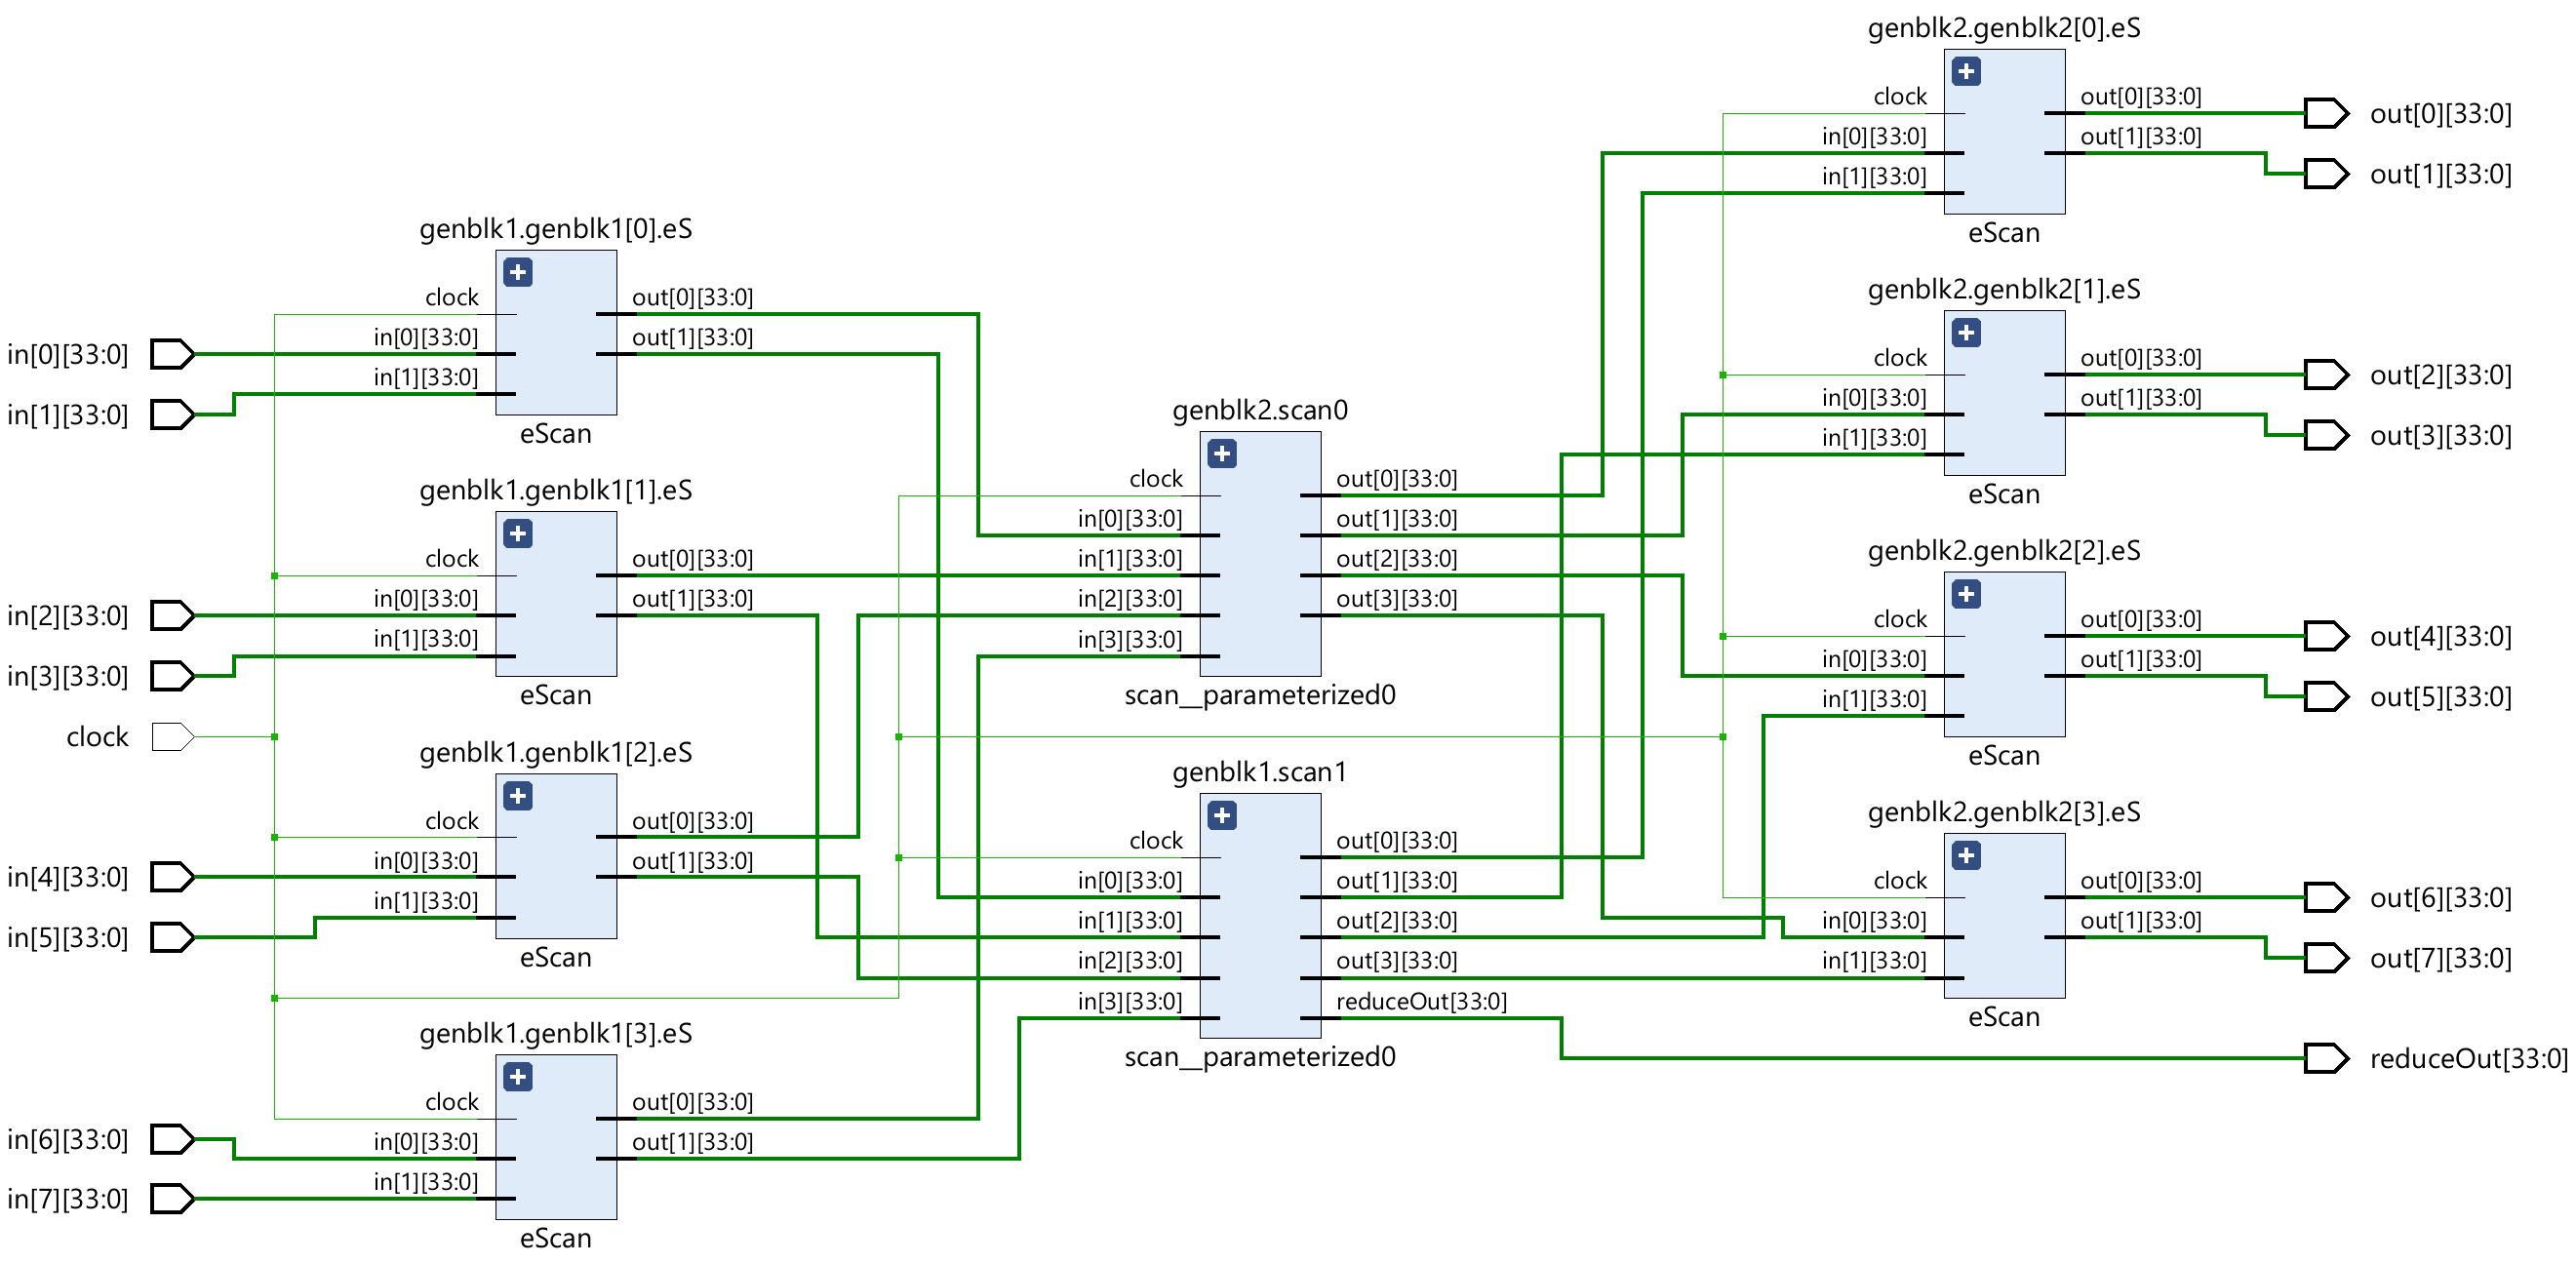
\includegraphics[width=\textwidth]{Images/scanRedTop.png}
    {\small {\bf a.}}
    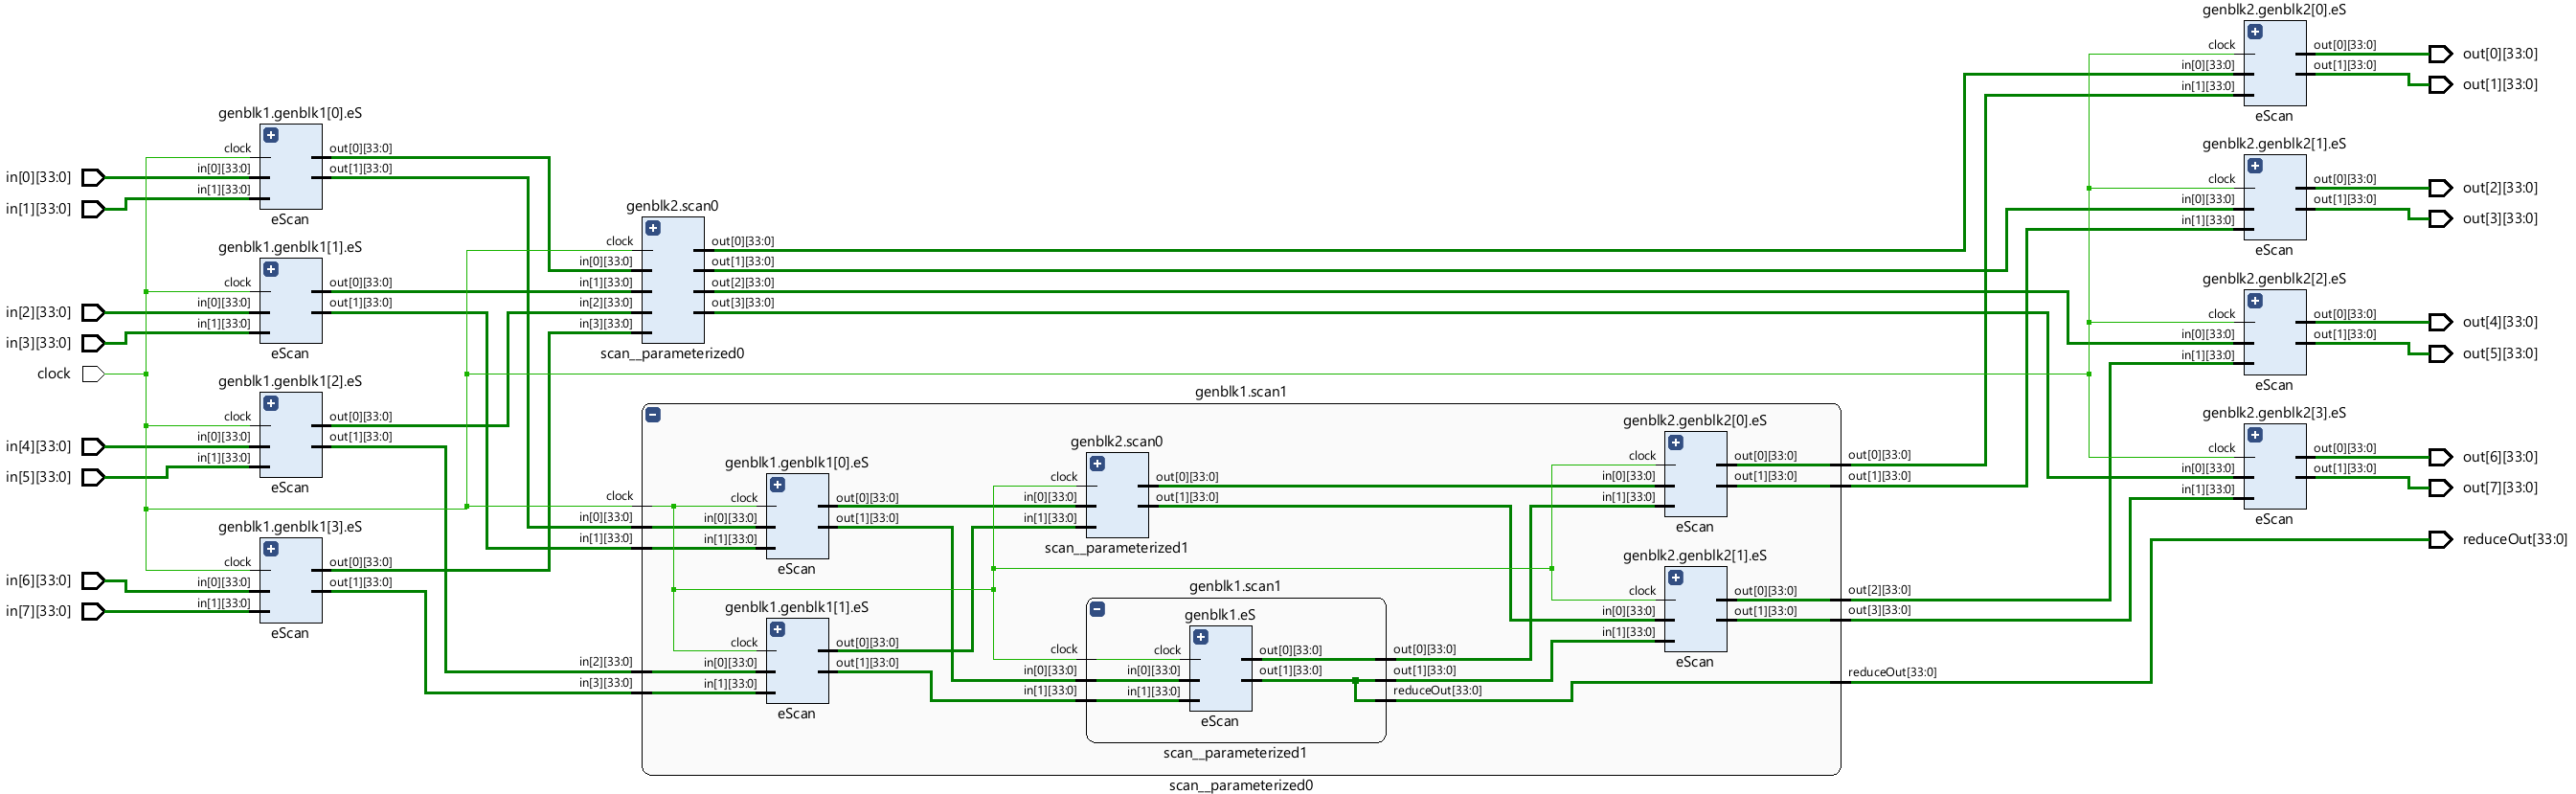
\includegraphics[width=\textwidth]{Images/scanRed.png}
   {\small  {\bf b.}}
    \caption{An 8-input scan circuit with the output for the reduction function. {\bf a}. The top module. {\bf b}. Detailed representation to emphasize {\tt reduceOut}. }
    \label{fig:scanRedTop}
\end{figure}

%\placedrawing[H]{figures/09_13_scan_net.lp}{ An 8-input scan circuit adapted for an 8-input prefix operation \cite{antonescu20} \cite{antonescu24}.} {red}

We use the term {\em scan} by extension, starting from the already established use for prefix-type networks.

\begin{definition}
Let be an associative and commutative  operation, {\tt OP}. OP-prefix computation is defined on the scalar vectors, $[s_0 \; s_1 \; \ldots \; s_{n-1}]$ and returns the vector $[p_0 \; p_1 \; \ldots \; p_{n-1}]$, where:
$$ p_i = OP_0^i s_i$$

$\diamond$
\end{definition}
\begin{exemplu}
For OP arithmetic sum we have addPrefix:
$$p_0 = s_0$$
$$p_1 = p_0 + s_1 = s_0 + s_1$$
$$p_2 = p_1 + s_2 = s_0 +s_1 + s_2$$
$$\ldots$$
$$p_{n-1} = p_{n-2} + s_{n-1} = s_0 + s_1 + \ldots \; s_{n-1}$$

$\diamond$
\end{exemplu}

{\bf Note}: the last output of $addPrefix$ is the output of $sumReduce$, thus justifying the simplified representation of the two loops in Figure \ref{secondLoop}.

The size of the pipeline implemented Scan network is in $O(p \times log \; p$, and the depth is in $O(log \; p$. Therefore, the size of the MapScanReduce structure is in $O(p \times log \; p$.

\subsection{Architectural additions}\label{scanEx}

The system architecture is completed by adding the second global loop, with  specific functions exemplified as follows:
\begin{description}
    \item[{\tt ADDPX(Vi)}:] add prefix returns a vector whose components are:\\
        $addPx_j \Leftarrow \sum_{j=0}^{j} (b_j ? s_{ij} : 0)$ for $j = 0, \ldots, p-1$ \\
         {\bf Example} of use: {\tt V2 <= ADDPX(V1)} 
    \begin{verbatim}
    For:        B  = [1 1 1 0 0 1 0 0]
                V1 = [2 3 1 4 3 5 2 0]
    results:    V2 = [2 5 6 6 6 11 11 11]
    \end{verbatim}
    \item[{\tt SPLIT(Vi)}:] return a vector with the selected components left aligned and the unselected component right aligned  \\
     {\bf Example} of use: {\tt V2 <= SPLIT(V1)} 
    \begin{verbatim}
    For:        B  = [0 1 1 0 0 1 0 0]
                V1 = [2 3 1 4 3 5 2 0]
    results:    V2 = [3 1 5 2 4 3 2 0]
    \end{verbatim}
\end{description}


\section{The mathematical model of partially recursive functions\index{partial recursive functions; defined by Stephen Kleene as a mathematical computational model}}

When we closed the fourth loop, starting from combinational circuits, we had the pleasant encounter with the mathematical model of the Turing Machine. Does a similar encounter await us with the closing of the two loops over a cellular automaton? Yes. It is a mathematical model proposed independently in the same year as the Turing Machine: the model of {\bf {\em partially recursive functions}} proposed by Stephen Kleene\index{Kleene, Stephen (1909-1994):  founder of  recursion theory, which subsequently helped to provide the foundations of theoretical computer science} \cite{Kleene36}.

\begin{definition}\label{parrec}
Let be the positive integers $x,y,i \in \mathbb{N}$ and the vector $\vec{x} = \langle x_0, x_1, \ldots, x_{n-1} \rangle \in \mathbb{N}^n$. Any partial recursive function $f: \mathbb{N}^n \rightarrow \mathbb{N}$ can be computed using three {\bf {\em initial functions}}:
\begin{itemize}
\item $ZERO(x) = 0:$ the variable $x$ takes the value {\bf zero}
\item $INC(x) = x+1:$ {\bf increment}s the variable $x \in \mathbb{N}$
\item $SEL(i, \vec{x}) = x_i:$ $i$ {\bf select}s the value of $x_i$ from the vector of positive integers $\vec{x}$
\end{itemize}
and the application of the following three {\bf {\em rules}}:
\begin{itemize}
\item {\bf Composition:}  $f(\vec{x}) = g(h_0(\vec{x}), \ldots, h_{p-1}(\vec{x}))$,
    where:  $f: \mathbb{N}^n \rightarrow \mathbb{N}$ is a total function if  $g: \mathbb{N}^p \rightarrow \mathbb{N}$ and  $h_i: \mathbb{N}^n \rightarrow \mathbb{N}$, for $i = 0,1, \ldots p-1$, are total functions
\item {\bf Primitive recursion:} $f(\vec{x},y) = g(\vec{x}, f(\vec{x}, (y-1)))$,  with $f(\vec{x},0) = h(\vec{x})$
    where:  $f:  \mathbb{N}^{n+1} \rightarrow  \mathbb{N}$ is a total function if $g:  \mathbb{N}^{n+1} \rightarrow  \mathbb{N}$ and $h:  \mathbb{N}^n \rightarrow  \mathbb{N}$ are total functions.
\item {\bf Minimization:} $f(\vec{x}) = \mu_y[g(\vec{x},y) = 0]$,
    which means: the value of the function  $f:  \mathbb{N}^{n} \rightarrow  \mathbb{N}$ is the smallest $y$, {\bf {\em if any}}, for which the function $g:  \mathbb{N}^{n+1} \rightarrow  \mathbb{N}$ takes the value $g(\vec{x},y) = 0$.
\end{itemize}

$\diamond$
\end{definition}

If we follow the previous definition, we will identify the initial functions with those directly realized by simple combinational circuits:
\begin{itemize}
    \item ZERO: implemented by generating a constant value
    \item INC: implemented as the increment circuit
    \item SEL: implemented as the multiplexer circuit
\end{itemize}
while the composition rule is implemented by the circuit represented in Figure \ref{compCirc}.

\placedrawing[h]{figures/14_9_compositionCircuit.LP}{{\bf The circuit version of composition.} {\small It is a two-layer construct: the parallel expanded {\em map} layer serially connected with the $log$-dept {\em reduction} layer.}}{compCirc}

The similarity between Figures \ref{firstLoop} and \ref{compCirc} encourages us to hope that both primitive recursion and minimization can find implementations in structures that we can physically realize with cellular constructions. Indeed, by composing {\em map composition} functions (see Figure \ref{compCirc}) one can obtain the purely theoretical construction in Figure \ref{2loops} (for details see \cite{Stefan00}). It is a theoretical one because is extended indefinitely to right for two reasons:
\begin{enumerate}
    \item we not know for how big $y$ a primitive recursion  computation is requested
    \item we not know for how big $y$, if any, the computation of a partial recursive function ends.
\end{enumerate}
While for the primitive recursion functions the value of $y$ is known at the beginning of computation, for the partial recursive functions the value of $y$, if any, is the result of the computation. For computing primitive recursive functions only  the map composition with the reduction network are sufficient, while for partial functions adding the scan network is mandatory. The simplest form of  the reduction network is one which provide the Boolean bitwise OR of the input components. For the scan network the minimal function receives a Boolean vector and provides the Boolean vector {\tt FIRST} which highlights only the first 1.

\placedrawing[h]{figures/14_10_partialRecursiveCircuit.lp}{{\bf The circuit version of the enhanced composition}. {\small In the map composition right connections are added considering specific map compositions. The scan circuit, a $log$-layer map compositions, is connected with the generic map composition.}}{2loops}

The theoretical structure in Figure \ref{2loops} can be transformed into an implementable one by adding a sequencer that converts the size of the structure into execution time. This becomes possible due to the local memories in each cell $M_i$. The result is a structure like the one in Figure \ref{secondLoop}, a structure that can be considered an {\bf {\em abstract model for a parallel computing system}}.


\section{Heterogeneous Computing\index{heterogeneous computing system: a host computer for the complex computation using a hardware accelerator for the intens computation}}

The main application of the MapScanReduce structure is in heterogeneous computing were the distinction between complex computing and intense computing is meaningful.

\subsection{Complexity vs. intensity in computation\index{complexity!complexity vs. intensity in computation}}

let's define the two types of computations. In this respect, we use the {\em algorithmic complexity} \cite{Chaitin70} which helps us make the necessary distinction between size and complexity.

\begin{definition}
The {\bf {\em algorithmic complexity}} of an entity is given by the length of its shortest description.

$\diamond$
\end{definition}

\begin{definition}
An entity is complex when its size is in the same magnitude order with its algorithmic complexity, and is simple when with a size in $O(f(N))$ its complexity remains in $O(1)$.

$\diamond$
\end{definition}

Now, regarding computation the following two definitions can be accepted.

\begin{definition}
Complex computation is characterized by an execution time proportional to the number of lines of executable code by which it is described.

$\diamond$
\end{definition}

\begin{definition}
The intensive, simple computation is described by a constant number, in $O(1)$, of lines of executable code, independent of the execution time which is in $O(f(N))$, where $N$ is used to define the size of the precessed data.

$\diamond$
\end{definition}

The previous definitions follow the algorithmic complexity \cite{Chaitin70} definition stating  mainly that the complexity of a computation is given by the length of its shortest description. While for complex computation the Turing tax can be reduced using {\em instruction-level parallelism}, for simple, intense computation a promising solution is  {\em cellular parallelism}. A typical example for intense, simple computation is the multiplication of $N \times N$ matrices performed on a mono-core engine in $O(N^3)$ time. An accelerator with $p$ execution units (cells) is expected to reduce execution times by at least $O(p/log \; p)$ times. It runs a constant (independent of N) code size.

\subsection{Heterogeneous system}\label{hetCompSystem}

Heterogeneous computing takes into account the distinction between complex and intensive computing. This segregation is possible using a system in which a single-core computer, instantiated as a HOST, uses a library of functions implemented in hardware in a MapScanReduce structure to perform complex calculations. In Figure \ref{hetSyst}, such a heterogeneous computing system is represented.

\placedrawing[h]{figures/09_10_heterogeneous_system.lp}{}{hetSyst}

The two types of computation, complex and intensive, can be performed efficiently if we have adequate hardware for each. This is what we achieve with a heterogeneous system. The problem is the acceleration that we obtain for an application in which we have a mixture of intensive and complex computation. Evaluating the performance of the accelerator is not enough because what is important is the total performance that is obtained by taking into account the execution time associated with the complex computation, which cannot be accelerated in the host, and the execution time associated with the intensive computation subject to acceleration in the accelerator.

Since the 1960s, with the advent of the first parallel computers, the problem of limited acceleration due to the weight of complex calculations has arisen. The limitation was expressed by Amdahl's Law.

Amdahl's law, named after  Gene Amdahl,  was introduced  at a conference in 1967 \cite{amdahl1967}, and can be used in parallel computing to predict the limit of the theoretical speedup when using heterogeneous computation. It is formulated in the following way:
$$A_{host+accelerator} = \frac{1}{(1-w_{intenseComp}) + \frac{w_{accelerator}}{A_{accelerator}}}$$
where:
\begin{description}
    \item[$A_{host+accelerator}$:] represents the overall acceleration of the heterogeneous system running an application
    \item[$A_{accelerator}$:] represents the acceleration obtained by the accelerator running the intense part of the application
    \item[$w_{intenseComp}$:] the weight of the intense computation in the application expressed by a subunit number
\end{description}
We can highlight two limiting cases:
\begin{enumerate}
    \item computation is dominated by the complex computation: with $w_{intenseComp} = 0.05$ and $A_{accelerator} = 1000$ results $A_{host+accelerator} = 1.05$
    \item computation is dominated by the intense computation: $w_{intenseComp} = 0.95$ and $A_{accelerator} = 1000$ results $A_{host+accelerator} = 19.62$
\end{enumerate}
In the limiting cases, for $w_{accelerator} = 1$ we have $A_{host+accelerator} = A_{accelerator}$, while for $w_{accelerator} = 0$ we have $A_{host+accelerator} = 1$.

\subsection{Programming a heterogeneous system}

Concerning the programming of multicellular processors, which have seen a rapid proliferation primarily driven by corporate considerations, the scientific community has yet to universally embrace effective solutions. The challenge arises from the prioritization of hardware criteria that promoted multi- and many-cell solutions without sufficient regard for their programmability. This is due to:
{\small
\begin{quote}
{\em "the semiconductor industry threw the equivalent of a Hail
Mary pass when it switched from making microprocessors run faster to
putting more of them on a chip—doing so without any clear notion of how
such devices would in general be programmed. The hope is that someone
will be able to figure out how to do that, but at the moment, the ball is still in the air."} \cite{Patterson10}
\end{quote}
}

%It seems that the solution is not specific languages for parallel structures:

It appears that the solution does not entail specific languages tailored for parallel structures:
{\small
\begin{quote}
{\em "The software span connecting applications to hardware relies more on parallel software architectures than on parallel programming languages. Instead of traditional optimizing compilers, we depend on autotuners, using a combination of empirical search and performance modeling to create highly optimized libraries tailored to specific machines."} \cite{Asanovic09}
\end{quote}
}

As a result, our heterogeneous approach imposes, for efficiency, a three level programming system:
\begin{enumerate}
    \item ACCELERATOR-level programming is done in assembly language providing a highly optimized library of primitives.
    \item HOST-level libraries  developed  in a high-level programming language  based on primitives provided by ACCELERATOR.
    \item HOST-level programming running  in a high-level programming language based on "highly optimized libraries tailored to specific machines".
\end{enumerate}

\subsubsection{Accelerator-level programming}

In Table \ref{ops} is listed partially the set of operations performed at the accelerator-level.


\begin{table}[h]
	\centering                       
	\caption{Accelerator-level operations}           
	\label{ops}       % Label

	\begin{tabular}{|l|l|} \hline  % Your table
		Operation & Description  \\ \hline \hline
        ACTIVATE    & activate all cells: $b_i=1$ for $i = 0,1,\ldots ,p1-$ \\ \hline
        WHERE(Vi=0) & where scalar in Vi is zero, cell remains active \\ \hline
        ELSEWHERE & cells inactivated by the last WHERE become active \\ \hline
        ENDWHERE & vector B takes the value before the most recent WHERE \\ \hline
		ADD(Vj,Vk) & add vectors Vj and Vk in each active position   \\ \hline
		MULT(Vj,Vk) & multiply vectors Vj and Vk in each active position   \\ \hline
        AND(Vj,Vk) & bitwise AND of vectors Vj and Vk in each active position  \\ \hline
        OR(Vj,Vk) & bitwise OR of vectors Vj and Vk in each active position  \\ \hline
        XOR(Vj,Vk) & bitwise XOR of vectors Vj and Vk in each active position  \\ \hline
        VAL(s) & generate a vector with value s in each active position \\ \hline
        ADDRED(Vi) & active components of Vi are submitted to reduction add \\ \hline
        MINRED(Vi) & active components of Vi are submitted to reduction minimum \\ \hline
        MAXRED(Vi) & active components of Vi are submitted to reduction maximum \\ \hline
        ORRED(Vi) & active components of Vi are submitted to reduction logic OR \\ \hline
        ADDPX(Vi) & active components of Vi are submitted to prefix add function \\ \hline
        SHIFTRIGHT(Vi, leftIn) & shift right the component of Vi and insert leftIn \\ \hline
        SHIFTLEFT(Vi, rightIn) & shift left the component of Vi and insert rightIn \\ \hline
        ROTATERIGHT(Vi) & rotate right the component of Vi \\ \hline
        ROTATELEFT(Vi) & shift left the component of Vi \\ \hline
	\end{tabular}

\end{table}


\subsubsection{Library of primitives: an example}\label{library}

One of the most used library of function contains linear algebra functions. In the following few of the most used linear algebra functions are described to exemplify the intense functions appropriate to be implemented on a MapScanReduce architecture.

\paragraph{Matrix} is a rectangular array of $n$ lines and $m$ columns scalar components, as follows:
\[
{\bf M} = \begin{bmatrix}
    s_{11} & s_{12} & s_{13} & \ldots & s_{1n} \\
    s_{21} & s_{22} & s_{23} & \ldots & s_{2n} \\
    \ldots & \ldots & \ldots & \ldots & \ldots \\
    s_{m1} & s_{m2} & s_[m3] & \dots  & s_{mn}
    \end{bmatrix}
\]

\paragraph{Identity matrix} is a matrix working as the scalar 1 in the arithmetic multiplication and division; it has 1s on the main diagonal as follows:
\[
{\bf I} = \begin{bmatrix}
    1 & 0 & 0 & \ldots & 0 \\
    0 & 1 & 0 & \ldots & 0 \\
    \ldots & \ldots & \ldots & \ldots & 0 \\
    0 & 0 & 0 & \dots  & 1
    \end{bmatrix}
\]

\paragraph{Row Vector} is a linear array of $n$ scalars, as follows:
\[
V = \begin{bmatrix}
    s_{1} & s_{2} & s_{3} & \ldots & s_{n} 
    \end{bmatrix}
\]

\paragraph{Column Vector} is a linear array of $m$ scalars, as follows:
\[
W = \begin{bmatrix}
    s_{1} \\
    s_{2} \\
    \ldots \\
    s_{m} 
    \end{bmatrix}
\]

\paragraph{Inner or dot product} of two vector provides a scalar as the sum of matching members products, as follows:
\[
V \cdot W = \begin{bmatrix}
    s_{1} & s_{2} & s_{3} & \ldots & s_{n} 
    \end{bmatrix}
    \cdot
    \begin{bmatrix}
    t_{1} \\
    t_{2} \\
    \ldots \\
    t_{n} 
    \end{bmatrix}
    = \sum_{1}^{n} s_i \times t_i
\]



\begin{exemplu} Let be the vectors {\tt V1 = [1 2 3 4]} and {\tt V2 = [5 6 7 8]}. Their inner, dot or scalar product is: $$V1 \cdot V2 = 1 \times 5 + 2 \times 6 + 3 \times 7 + 4 \times 8 = 70$$

$\diamond$
\end{exemplu}

\paragraph{Matrix-vector multiply} provide a vector of the dot products between the lines of the matrix and the vector, as follows:

\[
{\bf M} \cdot W = \begin{bmatrix}
    s_{11} & s_{12} & s_{13} & \ldots & s_{1n} \\
    s_{21} & s_{22} & s_{23} & \ldots & s_{2n} \\
    \ldots & \ldots & \ldots & \ldots & \ldots \\
    s_{m1} & s_{m2} & s_[m3] & \dots  & s_{mn}
    \end{bmatrix}
    \cdot
    \begin{bmatrix}
    t_{1} \\
    t_{2} \\
    \ldots \\
    t_{n} 
    \end{bmatrix}
    = 
    \begin{bmatrix}
    V_{1} \\
    V_{2} \\
    \ldots \\
    V_{m} 
    \end{bmatrix}
    \cdot W
    = 
    \begin{bmatrix}
    V_{1} \cdot W \\
    V_{2} \cdot W \\
    \ldots \\
    V_{m} \cdot W
    \end{bmatrix}
\]


\begin{exemplu}
Let be the matrix
\[
M = \begin{bmatrix}
    1 & 2 & 3 \\
    4 & 5 & 6\\
    7 & 8 & 9
    \end{bmatrix}
\]
and the vector 
\[
V = \begin{bmatrix}
    10 \\
    11 \\
    12 
    \end{bmatrix}
\] 
their product is:
\[
M \times V = \begin{bmatrix}
    1 & 2 & 3 \\
    4 & 5 & 6\\
    7 & 8 & 9
    \end{bmatrix}
    \cdot
    \begin{bmatrix}
    10 \\
    11 \\
    12
    \end{bmatrix}
    = 
    \begin{bmatrix}
    1 \times 10 + 2 \times 11 + 3 \times 12 \\
    4 \times 10 + 5 \times 11 + 6 \times 12  \\
    7 \times 10 + 8 \times 11 + 9 \times 12 
    \end{bmatrix}
    = 
     \begin{bmatrix}
    68 \\
    167 \\
    326
    \end{bmatrix}
\]

$\diamond$
\end{exemplu}

\paragraph{Matrix multiplication} of two matrices ${\bf M_1}$ and ${\bf M_2}$ provides a matrix ${\bf M}$ whose lines a contains the dot products of a column, starting with the first column, form ${\bf M_2}$ with each lines from ${\bf M_1}$ starting with the first line in ${\bf M_1}$. The number of lines in ${\bf M_1}$ must be the same with the number of columns in ${\bf M_2}$. The general form is:

\[
{\bf M_1} \cdot {\bf M_2} = 
    \begin{bmatrix}
    s_{11} & s_{12} & s_{13} & \ldots & s_{1k} \\
    s_{21} & s_{22} & s_{23} & \ldots & s_{2k} \\
    \ldots & \ldots & \ldots & \ldots & \ldots \\
    s_{m1} & s_{m2} & s_[m3] & \dots  & s_{mk}
    \end{bmatrix}
    \cdot
    \begin{bmatrix}
    t_{11} & t_{12} & t_{13} & \ldots & t_{1n} \\
    t_{21} & t_{22} & t_{23} & \ldots & t_{2n} \\
    \ldots & \ldots & \ldots & \ldots & \ldots \\
    t_{k1} & t_{k2} & t_[k3] & \dots  & t_{kn}
    \end{bmatrix}
    =
\]
\[
    =
    \begin{bmatrix}
    V_{1} \\
    V_{2} \\
    \ldots \\
    V_{m} 
    \end{bmatrix}
    \cdot
    \begin{bmatrix}
    W_{1} & W_{2} & W_{3} & \ldots & W_{n} 
    \end{bmatrix}
    =
    \begin{bmatrix}
    V_{1} \cdot W_{1} & V_{1} \cdot W_{2} & V_{1} \cdot W_{3} & \ldots & V_{1} \cdot W_{n} \\
    V_{2} \cdot W_{1} & V_{2} \cdot W_{2} & V_{2} \cdot W_{3} & \ldots & V_{n} \cdot W_{n} \\
    \ldots & \ldots & \ldots & \ldots & \ldots \\
    V_{m} \cdot W_{1} & V_{m} \cdot W_{2} & V_{m} \cdot W_{3} & \ldots & V_{m} \cdot W_{n} 
    \end{bmatrix}
\]


Let us consider the simplest, most intense computation of multiplying matrices.
\includeverilogcode[caption={Matrix multiplication in Python.  File: matrix\_multiplication.py. }, 
                    label={lst:matrixMultiplication}, 
                    firstline=1, 
                    firstnumber=1, 
                    lastline=68]
                    {\verilogSourceDir/A14_matrix_multiplication.py}

The execution time of this program on a mono-core processor is proportional with the number of clock cycles:
$$range(cols\_B) \times range(cols\_B) \times range(cols\_A)$$
which means, for example: if $range(cols\_B) = range(cols\_B) = range(cols\_A) = 1024$, the execution time is proportional with $1024^3 \simeq 10^9$.

However, in high-level languages like Python there are function libraries for frequently used functions like matrix multiplication. In this case the program takes the simplified form below:
\includeverilogcode[caption={Matrix multiplication in Python using a library of function.  File: matrixMultiplication.py. }, 
                    label={lst:matrixmultiplication}, 
                    firstline=1, 
                    firstnumber=1, 
                    lastline=68]
                    {\verilogSourceDir/A14_matrixMultiplication.py}

The line {\tt result = np.dot(A,B)} access, when the program runs on a mono-core processor, a highly optimized program (usually written in assembly language) for the matrix multiplication operation. In a heterogeneous system, instead of calling a program from library, is accessed a function performed hardware accelerated by the associated accelerator.

\begin{exemplu}
Let see how looks the algorithm for multiplying two $n \times n$ matrices, {\tt A} and {\tt B}. The transposed matrix of B is {\tt T}. Each matrix is represented by vectors in a Map with $p\geq n$.
{\em 
\includeverilogcode[caption={Matrix multiplication algorithm using a hardware accelerator.  }, 
                    label={lst:matrixMult}, 
                    firstline=1, 
                    firstnumber=1, 
                    lastline=68]
                    {\verilogSourceDir/A14_matrixMult}
}

Because the previous algorithm works with vectors, instead of the three embedded lops in the Python program {\tt matrix\_multiplication.py}, in the {\tt matrix\_multiplication} algorithm {\bf {\em there are only two embedded loops}}. Besides this good news, there is also a bad news: the operation repeated $n^2$ times is executed in time belonging to $O(log \; n)$ cycles. Because the line {\tt result[i][j] += A[i][k] * B[k][j]} in the Python program is executed in constant time, the acceleration provided by the MapScanReduce accelerator is only of $n/log_2 n$. (A well-designed algorithm can avoid this bad news, but this topic goes beyond the level at which we approach parallelism problems.)

$\diamond$
\end{exemplu}

\paragraph{Matrix transpose} applied to the matrix $M$ is $M^T$ with the lines equal with the columns of $M$.

\begin{exemplu}
Let be the matrix:
\[
M = \begin{bmatrix}
    1 & 2 & 3 \\
    4 & 5 & 6\\
    7 & 8 & 9
    \end{bmatrix}
\]
Its transpose is:
\[
M^T = \begin{bmatrix}
    1 & 4 & 7 \\
    3 & 5 & 8\\
    3 & 6 & 9
    \end{bmatrix}
\]

$\diamond$
\end{exemplu}

To describe the algorithm for square matrix transpose, we will define the concept of {\bf {\em pseudo diagonal}} of a square matrix.

\begin{definition}
{\em
Let be the square matrix
\[{\bf M} =
\begin{bmatrix}
    v_{00} & v_{01} & \dots  & v_{0 \; m-1}\\
    v_{10} & v_{11} & \dots  & v_{1 \; m-1}\\
    \vdots & \vdots & \ddots & \vdots\\
    v_{m-1 \; 0} & v_{m-1 \; 1} & \dots  & v_{m-1 \; m-1}
    \end{bmatrix}
\]
where $$PD(k,{\bf M}) = [v_{(0+k)_{mod \; m} \; 0} \; v_{(1+k)_{mod \; m} \; 1} \ldots v_{(m-1+k)_{mod \; m} \; m-1}]$$ is the $k$-th {\bf {\em pseudo-diagonal}} in the matrix {\bf M}. (The 0-th pseudo-diagonal is the main diagonal.)
}

$\diamond$
\end{definition}

A vector algorithm for matrix transpose uses the pseudo-diagonal concept, as follows:

{\footnotesize
\begin{shaded*}
\begin{lstlisting}[language=Verilog, caption= , morekeywords={activate, where, wait, loop, repeat, doInParallel, for}]
/*******************************************************************************
    Algorithm for matrix transpose
        Initial matrix, V, with components: v(i,j), for i,j = 0, 1, ... m-1
        Final matrix, W, with components:   w(i,j), for i,j = 0, 1, ... m-1
        Working vector: A = [a(0) a(1) ... a(m-1)]
    Note: addition and subtract operations are modulo m operations
********************************************************************************/
for(k=0; k<m; k=k+1) begin
  (step 1) A <= [v(0+k,0)v[1+k,1]...v[m-1+k,m-1] // A <= PD(k.V)
  (step 2) A <= [a(0-k)a(1-k)...a(m-1-k)]        // A <= (A rotate k times right)
  (step 3) for(j=0; j<m; j=j+1) w(j+k,j) <= a(j) // PD(m-k,W) <= A
end
\end{lstlisting}
\end{shaded*}
}


\begin{exemplu}
Let's consider the $4 \times 4$ matrix V. Its transposed form is computad as follows:

{\small
\begin{verbatim}
    Initial                                                        Final
                          k = 0    k = 1    k = 2    k = 3
 V: 0 1 2 3     (step 1) 0 5 A F  4 9 E 3  8 D 2 7  C 1 6 B     V: 0 1 2 3
    4 5 6 7                                                        4 5 6 7
    8 9 A B                                                        8 9 A B
    C D E F                                                        C D E F

                (step 2) 0 5 A F  3 4 9 E  2 7 8 D  1 6 B C

 W: x x x x     (step 3) 0 x x x  0 4 x x  0 4 8 x  0 4 8 C     W: 0 4 8 C
    x x x x              x 5 x x  x 5 9 x  x 5 9 D  1 5 9 D        1 5 9 D
    x x x x              x x A x  x x A E  2 x A E  2 6 A E        2 6 A E
    x x x x              x x x F  3 x x F  3 7 x F  3 7 B F        3 7 B F
\end{verbatim}
 }

$\diamond$
\end{exemplu}




\begin{exemplu}
In Table \ref{prim} is listed an example for a library of primitives:  FLA 0.1. It can be used to develop in a high level language on HOST a linear algebra library. The library of primitives contains functions defined on data structures -- vectors and matrices --- limited to the size of the array of cells  Map, i.e., $p$-component vectors and $p \times p$ matrices. Programs developed on HOST adapt linear algebra operations defined on data of any size to linear algebra operations defined on accelerator dimensions. In this way, a speedup is obtained that depends on $p$ even if the order of magnitude of the computation time remains the same, i.e., the execution time of matrix multiplication, for example, remains the same, in $O(n^3)$ for matrices of $n \times n$.

{\em
\begin{table}[H]
	\centering                       
	\caption{Library of linear algebra primitives, FLA 0.1,  for $p \times p$ matrices and $p$-component vectors on a $p$-cell MapScanReduce accelerator. }           
	\label{prim}       % Label
	\begin{tabular}{|p{0.22\textwidth}|p{0.55\textwidth}|p{0.075\textwidth}| } \hline  % Your table
		{\bf FLA 0.1 functions}    & {\bf Description}                                 & {\bf Time}  \\ \hline \hline
        hSTART            & start the cycle counter on sequencer's            & $O(1)$ \\ \hline
        hSTOP             & stop the cycle counter on sequencer's             & $O(1)$ \\ \hline
        hINTRQ            & interrupt request                                 & $O(1)$ \\ \hline
        hVGENN(d,v)       & generate in V(d) uniform vector, [v v ... v]                                    & $O(1)$ \\ \hline
        hVGENX(d)         & generate in V(d) index vector, [0 1 ... p-1]                                    & $O(1)$ \\ \hline
        hMAIN(d,v)        & generate, starting with V(d), matrix with main diagonal of values v             & $O(p)$ \\ \hline
        hSQGENN(d)        & generate, starting with V(d) = [0 0 ... 0], matrix with incremental lines       & $O(p)$ \\ \hline
        hSQGENX(d)        & generate, starting with V(d) = [0 1 ... p-1], matrix with incremental lines     & $O(p)$ \\ \hline
        hPRANDOM(d)       & generate, starting with V(d), pseudo-random matrix                              & $O(p)$ \\ \hline
        hMSEND(a,s)       & send to host a s-line matrix starting with V(a)                                 & $O(ps)$ \\ \hline
        hMGET(a,s)        & get from host a s-line matrix starting with V(a)                                & $O(ps)$ \\ \hline
        hTRANS(d,l)       & transpose matrix starting at V(l) in matrix starting at V(d)                    & $O(p^2)$ \\ \hline
        hSQMADD(d,l,r)    & add starting from V(d) the matrices starting from V(l) and V(r)                 & $O(p)$ \\ \hline
        hSQMVMULT(m,v,d)  & multiply in V(d) the matrix starting at V(m) with the vector V(v)               & $O(p)$ \\ \hline
        hSQMMULT(d,l,r)   & multiply in matrix starting with V(d) matrices starting with V(l) and V(r)      & $O(p^2)$ \\ \hline
        hSQMMAC(d,l,r)    & multiply and add in matrix starting with V(d) matrices starting with V(l) and V(r)      & $O(p^2)$ \\ \hline
	\end{tabular}
\end{table}
}

$\diamond$
\end{exemplu}

\begin{exemplu}
Let us consider an accelerator with $p=256$ and the program for multiply $1024 \times 1024$ matrices. Then, the HOST consider the multiplication of matrices of $4 \times 4$ matrices of $256 \times 256$ components. The acceleration compared to the computation without accelerator is:
$$\alpha = \frac{k_1 \times 1024^3}{k_2 \times 4^3 \times k_3 \times 256^2} = k \times 256 \in O(p)$$

$\diamond$
\end{exemplu}

\section{Parallel Computing Patterns\index{parallel computing patterns!}}

Multiplying matrices is a promising example for the capacity to perform in parallel with MapScanReduce accelerator intense computation. It would be interesting to investigate the acceleration capacity of the MapScanReduce framework for a wider range of applications. A good idea could be formed by looking at the computational patterns that have been highlighted in applications designed and run in the last decades. Let us start with the study carried out in \cite{McCool12} from which we use Figure \ref{parallelPatt} where 17 parallel computational patterns are presented. We will see that almost all of them can be performed using the accelerator MapScanReduce. We will not succeed in the case of those patterns that do not represent an intensive computation but a complex one.

\placedrawing[h]{figures/09_14_parallelPatterns.lp}{Parallel patterns \cite{McCool12}.}{parallelPatt}

We will analyze in turn how the 17 patterns revealed by McCool and his collaborators can be accelerated using the MapScanReduce structure. These patterns classifies in three categories:
\begin{enumerate}
    \item Map-Only patterns -- executed on {\bf {\em no global loop}} structure
    \begin{enumerate}
        \item Map-Reduce patterns -- executed on {\bf {\em one global loop}} structure
        \item Map-Scan -- executed on {\bf {\em one global loop}} structure
    \end{enumerate}
    \item Map-Scan-Reduce -- executed on {\bf {\em two global loops}} structure
\end{enumerate}

\subsection{Patterns with Map-Only Implemented with No Global Loop}

A first subset of patterns is the one that are implementable with the Controlled Cellular Automaton (see \ref{contrCellAut}) structure used as accelerator. Many of the patterns we consider are executed exclusively involving the Map section. For them to be executed, a sequence of Map operations is required each time.

\subsubsection{Map Pattern\index{parallel computing patterns!map pattern}}

From the list proposed by McCool \& Co., the Map pattern finds a direct counterpart in the accelerator we are evaluating. In Figure \ref{parallelPatt} the Map pattern is represented using green boxes, which represent data, and blue boxes, which represent hardware structure performing sequences of $bOp$s and $uOp$s. Overall the array of blue boxes represents a Map structure performing a {\tt MAPOP(Va,Vb,Vc,...)} on the vectors stored along the cells of the array. Thus, the Map pattern is has a direct correspondent in we can do with arithmetic \& logic vector operations. 

\begin{exemplu}
Let be an $8$-cell Map with 
\begin{verbatim}
    V10 = <x x x x x x x x>
    V12 = <2 4 7 1 8 4 5 2>
    V15 = <4 2 2 8 5 1 3 6>
\end{verbatim}
and we have to generate in the even indexed cells of V10 the sum of  the even indexed cell from V12 and V15 and in odd cells of V10 the difference between the odd cells of V12 and V15. The sequence of operations is:
\begin{verbatim}
    ACTIVATE            | B = <1 1 1 1 1 1 1 1>: set all cells active
    V2 <= VAL(1)        | V2 = <1 1 1 1 1 1 1 1>: load 1 in all positions of V2
    V3 <= AND(IX,V2)    | V3 = <0 1 0 ... 1>: bwAND between IX and V2 
    WHERE(V3==0)        | B = < 1 0 1 ... 0>
    V10 <= ADD(V12,V15) | V10 = <6 x 9 x 13 x 8 x>
    ELSEWHERE           | B = <0 1 0 ... 1> 
    V10 <= SUB(V12,V15) | V10 = <6 2 9 -7 13 3 8 -4>
    ENDWHERE            | B = <1 1 1 1 1 1 1 1>
\end{verbatim}
The execution time of the previous sequence of operations does not depend on the number of cells, i.e., the execution time is in $O(1)$. The acceleration provided by this execution, compared with one performed by a mono-core engine, is in $O(p)$. The degree of parallelism si near 1, i.e., almost  in each clock cycle all cells are active. 

$\diamond$
\end{exemplu}

There are real premises for the acceleration obtained by using a Map array to be in $O(p)$, but more than that there are many cases when the acceleration is  {\bf {\em superlinear}} compared to a single-core structure, due to the control that is performed by SQ, control that in a single-core implementation is also the responsibility of the processor \cite{antonescu24a}.

\subsubsection{Stencil Pattern\index{parallel computing patterns!stencil pattern}}

The stencil pattern (depicted in  Figure \ref{parallelPatt}) is not directly implemented in the structure of the proposed accelerator, but can be efficiently programmed taking into account the fact that the input data structure is a matrix that can be loaded as part of the ${\bf M_{mp}}$ matrix. The finite neighborhood of each cell can be involved in the calculation of a new value in each cell very efficiently, because the values from the vertical vectors are in the same cell and a global shift operations allows access to the values from the horizontal vector. In fact, any finite neighborhood can be involved in updating  any value in ${\bf M_{mp}}$.

For example, let us consider the matrix stored in vectors from $V_0$ to $V_{n-1}$. Let us  consider a stencil computation in each cell of vector $V_i$ using as operands values from a type of neighborhood emphasized in Figure \ref{parallelPatt}: $s_{ij}$ as a central value, $s_{i(j-1)}, s_{i(j-2)}$ as values from the same vector positioned left, and $s_{i(j+1)}, s_{i(j+2)}$ positioned right, $s_{(i+1)j}, s_{(i+2)j}, s_{(i-1)j}, s_{(i-2)j}$ positioned in the same cell up two positions and down two positions.  The values to be used as operands are collected  in each cell and then submitted to a pure map sequence of operations which update the horizontal vector $V_i$ as follows:
\begin{verbatim}
    Vn     <= SHIFTRIGHT(Vi,0)
    V(n+1) <= SHIFTRIGHT(Vn,0)
    V(n+2) <= SHHIFTLEFT(Vi,0)
    V(n+3) <= SHHIFTLEFT(V(n+2),0)
    MAPOP(Vi,Vn,V(n+1),V(n+2),V(n+3),...)
\end{verbatim}
Because the update computation is done in parallel  for all the components of the horizontal vector $V_i$, the acceleration of the computation is in $O(p)$.

\subsubsection{Geometric Decomposition  Pattern\index{parallel computing patterns!geometric decomposition pattern}}

The geometric decomposition pattern works on configurable (overlapping) sub-collections  of data. In Figure \ref{parallelPatt}, four $5 \times 5$ scalars sub-collections are defined. If data is loaded in the accelerator's memory as a matrix of scalars, a sub-collection, $S(i,j,k,q)$, is a matrix loaded in ${\bf M_{mp}}$ between two horizontal vectors , $V_i$ and $V_j$, and two columns (vertical vectors), $C_k = [s_{0k} \; s_{1k} \ldots s_{m-1 \; k}]$ and $C_q = [s_{0q} \; s_{1q} \ldots s_{m-1 \; q}]$. The values for $i$ and $j$ are controlled by the program executed on the sequencer SQ, while the values of $k$ and $q$ are used by the {\em spatial selection} mechanism in Map. The $IX$ vector is used to delimit the index  of the vertical vectors applying spatial selection functions:
\begin{verbatim}
    WHERE(IX>=k)
    WHERE(IX<=q)
    MAPOP(Vi,V(i+1), ... V(j-1),V(j))
\end{verbatim}
Thus, any sub-collection is delimited in the matrix ${\bf M_{mp}}$, if $i,j,k,q \leq m,p$, in constant time. The degree of parallelism depends on the size of the sub-collections.

\subsubsection{Partition  Pattern\index{parallel computing patterns!partition pattern}}

The partition pattern corresponds to a geometric decomposition pattern without overlapping regions. See in Figure \ref{parallelPatt} a partition in four $4 \times 4$ scalars sub-collections. When dealing with sub-collections of varying sizes, it involves  {\em segmentation}. The same mechanisms for defining sections (sub-collections) used for geometric decomposition are considered for splitting, with the additional care to avoid overlap. We can take into account for the horizontal delimitations, in addition to those stated for the geometric decomposition, conditions imposed on the content of the horizontal vectors. The spatial selection functions, specific to the MAP structure, represent a particularly useful feature, specific to MapScanReduce architecture.

\subsubsection{Speculative Execution Pattern\index{parallel computing patterns!speculative execution pattern}}

Within a many-cell system, the speculative selection pattern is an optimization technique which  performs both computations and multiple-condition evaluations, in order to combine condition evaluation with processing. On our machine it is executed as a map pattern involving a {\tt MAPOP(...)} followed by various spatial selections.

\begin{exemplu}
Let there be a Boolean expression of $log_2 p$ binary variables and we are required to determine the binary configurations for which the expression takes the logical value 1. The binary form of the index of each cell in the Map represents the $p$ binary combinations for which the expression must be evaluated. The cells evaluate in parallel the same expression under the SQ command and finally using spatial selection the cell in which the evaluation result is 1 remains active.

$\diamond$
\end{exemplu}

The acceleration obtained for this  pattern is in $O(p)$.

\subsubsection{Recurrence Pattern\index{parallel computing patterns!recurrence pattern}}

The recurrence pattern represented in the expanded form   in  Figure \ref{recurrence} is characterized by nested loops with data dependencies. These structures can be parallelized by obtaining a dependency graph and creating tasks that can be run in parallel for each layer of the graph (separating hyperplane).

\placedrawing[h]{figures/09_15_recurrence_pattern.LP}{Recurrence pattern implementation  \cite{McCool12}.}{recurrence}

Since the recurrence pattern appears in loops, where operations are repeated, these can be run on our machine as all cells will execute the same instructions. Moreover, the fixed and predetermined data access pattern further facilitates this process.

Let us consider, as example the $p \times p$ recurrence pattern depicted in Figure \ref{recurrence} for $p=4$ (see in \cite{McCool12} at pag. 206). The computation consists of $p$ cycles. In each cycle, a scalar, {\tt si}, for $i = 0,1,...,p-1$ is inserted in a vector in  Map and the resulting vector is involved in a MAPOP processing. In each cycle the MAPOP sequence can be different. The sequence of operations for a certain computation is, in our MapScanReduce accelerator, the following:
\begin{verbatim}
    V1 <= SHIFTRIGHT(V1,s1)
    MAPOP(V1,...)
    V2 <= SHIFTRIGHT(V2,s2)
    MAPOP(V2,...)
    V3 <= SHIFTRIGHT(V3,s3)
    MAPOP(V3,...)
    V4 <= SHIFTRIGHT(V4,s4)
    MAPOP(V4,...)
    ...
    Vp <= SHIFTRIGHT(Vp,s(p))
    MAPOP(Vp,...)
\end{verbatim}

In time in $O(p)$ a number of operations in $O(p^2)$ are performed, thus obtaining an acceleration in $O(p)$.


\subsubsection{Pipeline  Pattern\index{parallel computing patterns!pipeline pattern}} 

The pipeline pattern refers to having a sequence of stages that flow into one another sequentially. Parallel speedup is achieved by ensuring that all stages carry out their respective operations independently of each other. In a departure from the traditional approach, this architecture implements the Pipeline principle as all major components (SQ, cells in Map, Scan/Reduce network, Data transfer mechanism) work in parallel to one another with data flowing between them.

The MapScanReduce architecture is suited for the pipeline pattern only when all computational cells must execute the same instructions, for situations where each pipeline stage executes the same operations, i.e., the pipeline of stages describes a simple, intense computation.

A typical example is the FIR filter computation involving the vectors V1 (to insert the input data in), V2 (to store the result of multiplications), V3 (to accumulate the results of multiplications), 4 (to store tap constants).
\begin{verbatim}
    loop{   V1 <= SHIFTRIGHT(V1,in)
            V2 <= MULT(V1,V4)
            V3 <= ADD(V3,V2)
            V3 <= SHIFTRIGHT(V3,0)  }
\end{verbatim}

The output of the computation is the right end of the vector V3.

A possible improvement is to combine the pipeline pattern with the reduce pattern. The loop will be shorted because the multiplication and the addition will be done in parallel in Map section and Reduce section of the MapReduce accelerator. The acceleration provided is in $O(p)$.

\subsection{Pattern Executable on MapReduce Only}

A second subset of patterns is that executed by structures containing a global reduction loop.

\subsubsection{Reduction Pattern\index{parallel computing patterns!reduction pattern}}

The reduction pattern is also performed directly by the proposed accelerator due to the Reduce network which is part of its hardware. The usual reduction functions are exemplified in subsection \ref{redEx}. They are executed directly by the hardware.

\subsubsection{Fork-Join  Pattern\index{parallel computing patterns!fork-join pattern}}

Fork-join is a control pattern that divides (fork)  work and subsequently combines (join) the results (see Figure \ref{parallelPatt}). This pattern is among the more general and loosely defined ones, making a comprehensive discussion challenging. As a starting point, two approaches can be brought to attention:
\begin{enumerate}
    \item simple symmetric patterns, a case of {\em divide et impera})
    \item complex, unpredictable, independent, thread spawning.
\end{enumerate}
Our accelerator can only be used  in the first case, which represents an intense, but simple computation.
The acceleration that can be obtained is in $O(p/log \; p)$ due to the latencies imposed by distribution, involved in fork, and reduction used to join the results.

\subsection{Pattern Executable on MapScan Only}

A third subset of patterns is that executed by structures containing the global scan loop.

\subsubsection{Scan Patterscan patternn\index{parallel computing patterns!scan pattern}}

 The scan pattern is also performed directly by the proposed accelerator due to the Reduce network which is part of its hardware. In subsection \ref{scanEx} two functions are exemplified. They are executed directly by the hardware.
 
\subsubsection{Pack Pattern\index{parallel computing patterns!pack pattern}}

The pack pattern is facilitated by the Scan section. The selection of the components to be packed is done using the Boolean vector $B$, which is managed by the spatial selection functions. The pattern is defined by  $B = \langle 0 \; 1\; 1\; 0\; 0\; 1\; 1\; 1 \rangle$. The positions in the destination vector of the components to be packed   are computed using the {\tt ADDPX(B)}. The algorithm is:
\begin{verbatim}
initially:  B  = <1 1 1 1 1 1 1 1>
            V0 = <0 1 1 0 0 1 1 1>
            V1 = <A B C D E F G H>

    WHERE(V0==1)        | B  = <0 1 1 0 0 1 1 1>
    V2 <= VAL(1)        | V2 = <x 1 1 x x 1 1 1>
    V2 <= ADDPX(V2)     | V2 = <x 1 2 x x 3 4 5>
    V2 <= ADD(V2,(-1))  | V2 = <x 0 1 x x 2 3 4>
    V3 <= PERM(V1,2)    | V3 = <B C F G H x x x>
    ENDWHERE
\end{verbatim}

The pack pattern is an operation accelerated in $O(p/log \; p)$ because of the latency introduced by the scan operations ({\tt ADDPX, PERM}).

\subsubsection{Gather  Pattergather patternn\index{parallel computing patterns!gather pattern}}

The gather pattern specifies in the source vector the source for each position in the destination vector (see Figure \ref{parallelPatt}). The gather pattern is a permutation defined using the order vector as its source and the index vector IX as its destination. We will denote by $(i)$ the content of the source or destination vector at position $i$.
In Figure \ref{parallelPattr}, the gather operation is defined by the operation permute with the order vector {\tt <(1)(5)(0)(2)(2)(4)>}.
Because the scalar C has two destinations, in the positions 2 and 3, the operation is performed in two steps using successively two order vectors: {\tt <(1)(5)(0)(2)(3)(4)>} and {\tt <(1)(5)(0)(2)(2)(4)>}.
Only if each destination has its distinct source, the operation is performed using one permutation operation. The acceleration for this pattern is in $O(p / log \; p)$, if the permutation is known in advance and control bits are precomputed.

\subsubsection{Scatter  Pattern\index{parallel computing patterns!scatter pattern}}

The scatter pattern specifies the destination for each position. The scatter pattern is a permutation defined using the index vector IX as its source and the order vector as its destination. In Fig. \ref{parallelPatt}:
\begin{center}
$ \langle  (0) \; (1) \; (2) \; (3) \; (4) \; (5) \rangle  \Rightarrow $
$\langle (1) \;  (5) \; (0) \; ({\bf 2}) \; ({\bf 2}) \; (4) \rangle  $
\end{center}
is represented as a deficient scatter because a destination, 2, has two distinct sources, 3 and 4. It must be considered a sort of ``overflow" and the system must generate an error (exception).

If the definition of scatter is not deficient, the scatter operation is a permute operation operated in the SCAN section of our accelerator with an acceleration in $O(p/log \; p)$, if the permutation is known in advance and control bits can be precomputed.

\subsubsection{Split  Pattern\index{parallel computing patterns!split pattern}}

The split pattern can be conceptualized as two sequential applications of the pack pattern. The first involves a standard pack with selected values going to the left, while the second necessitates computing the $NOT (B)$ vector such that previously unselected values are now selected and can then be packed to the right using {\tt COMPRIGHT(d,l,r)}. In {\tt sequence of operations} for pack pattern the vector {\tt v0} is complemented, instead {\tt VSUB(2,2,1)} is executed {\tt VADD(2,2,(p-REDMAX(V2)-1))} followed by {\tt COMPRIGHT(V2,V1,V2)}.

As with pack, the split pattern is accelerated in $O(p/log \; p)$.

\subsubsection{Expand  Pattern\index{parallel computing patterns!expand pattern}}

For this pattern each cell stores a self-delimited vertical vector of size $0$ to $p$ (refer to  Figure \ref{parallelPatt}).

The expand  pattern is implemented in three steps:
\begin{enumerate}
    \item the matrix ${\bf M_{mp}}$ is transposed (an efficient algorithm uses permutation)
    \item the resulting empty lines are removed
    \item the resulting self-delimited horizontal vectors are transferred serially to the sequencer's memory.
\end{enumerate}

Due to the serial transfer of data to the sequencer's memory, this pattern cannot be accelerated on this architecture. This time the complexity is given by the data structure, even if the algorithm is in the category of intense, simple ones.


\subsection{Patterns Executable on MapScanReduce}

There follow  a pattern that assume the use of the entire structure of the accelerator MapScanReduce.

\subsubsection{Category Reduction Pattern\index{parallel computing patterns!category reduction pattern}}

Category reduction pattern selects the set of elements that make up the string stored in a number of horizontal vectors,  is not directly implemented in the structure of the proposed accelerator, but it can be efficiently programmed. We consider that  the ${\bf M_{mp}}$ matrix distributed within the Map section has the capability to store the input stream $S$, which has the  of length $|S|$ in the form of  $N = \lceil |S|/p \rceil$ $p$-component vectors.

Spatial selections are utilized to keep active only cells where the vector Vi, for $i = 1, 2, ...,N$, has no $x$s, a value not included in $S$.  The same operation allows the selection of all cells where the remained active calls contain $F$ the first value different from $X$ which is and substitute it with $X$. The result is the stream $R$ in D, initially empty. The sequence of operations is:
\begin{verbatim}
    R = <>
    for(i=1; i=<N; i=i+1) {
      do on Vi   WHERE(!== x)
                 WHERE(first)
                 v0 <= REDADD(Vi)
                 R <= <R v0>
                 for(j=i; j<N; j=J+1) {
                    do on Vj    WHERE(v0)
                                VAL(x)     
                 }
      until(Vi = <X,X,...,X>)              
    }
\end{verbatim}

Because the mono-core execution of the pattern has the time in $O(|S| \times |D|)$, and the execution time in our accelerator is in $O(|S|/p \times |D| \times log \; p)$, the acceleration obtained for this pattern is in $O(p/log \; p)$. The  $log$ part in our evaluation appears due to the latencies of Scan to determine the first occurrence of a symbol different from $X$ in a vector $V_j$ (see line {\tt WHERE(first)}, and due to the latency of Reduce network to read in Controller the value of the first occurrence different from $x$ in the vector Vi) (see line {\tt v0 <= REDADD(Vi)}).

Important note: the scan type network used for this pattern processes a Boolean vector, which is why we can approximate that the size of the system remains in $O(p)$.

\subsection{Super-scalar Sequence Pattern\index{parallel computing patterns!super-scalar pattern}}

The super-scalar pattern describes a complex computation, which is why it requires a special discussion. The content of the square boxes in Figure \ref{parallelPatt} can be:
\begin{enumerate}
\item a simple instruction or a complex sequence of instructions
\item a complex computation performed on a data structure with size in $O(f(N))$.
\end{enumerate}
In the first case, the solution is  instruction-level parallelism competence and the implementation is done with a super-scalar pipeline processor. In the second case, the solution can be provided by the recently introduced concept of accelerator-level parallelism (ALP) \cite{HillReddi21} \cite{Malita22}.

A way of implementing ALP can be a MapScanReduce system with cells as MapScanReduce structures. Each cell accelerates an intense function that can be different from the others. We can say that a {\em super-tensorial} computation is ensured. We are dealing with a complex calculation that involves intensive calculations.

\section{Problems}

\begin{problem}
Simulate 64 cycles the cellular automaton defined in Example \ref{lb:cellAut} for $n=127$ in three versions:
\begin{enumerate}
    \item {\tt func  = 01011010 } and {\tt init = 1'b1 << 63}
    \item {\tt func  = 00011110 } and {\tt init = 1'b1 << 63}
    \item {\tt func  = 10100110 } and {\tt init = 4'b1001 << 61}
\end{enumerate}
Explain, for the third case, the periodic reappearance of the initial pattern duplicated each time.

$\diamond$
\end{problem}

\begin{problem}
Design for $p$ and simulate for $p=16$ the distribution network represented in Figure \ref{distribute}.

$\diamond$
\end{problem}


    
{\bf Solution}

For the circuit description to be valid for any $p$ we will need to make a recursive description using the {\bf {\em conditional generate}} structure. In Listing \ref{lst:distribute} we use the elementary module defined in Listing \ref{lst:elDistribute} and the distributor with $p$ destinations is defined using the distributor for $p/2$ destinations.

\includeverilogcode[caption={Distribution network.  File: distribute.sv. }, 
                    label={lst:distribute}, 
                    firstline=1, 
                    firstnumber=1, 
                    lastline=68]
                    {\verilogSourceDir/A14_distribute.sv}

\begin{figure}[H]
    \centering
    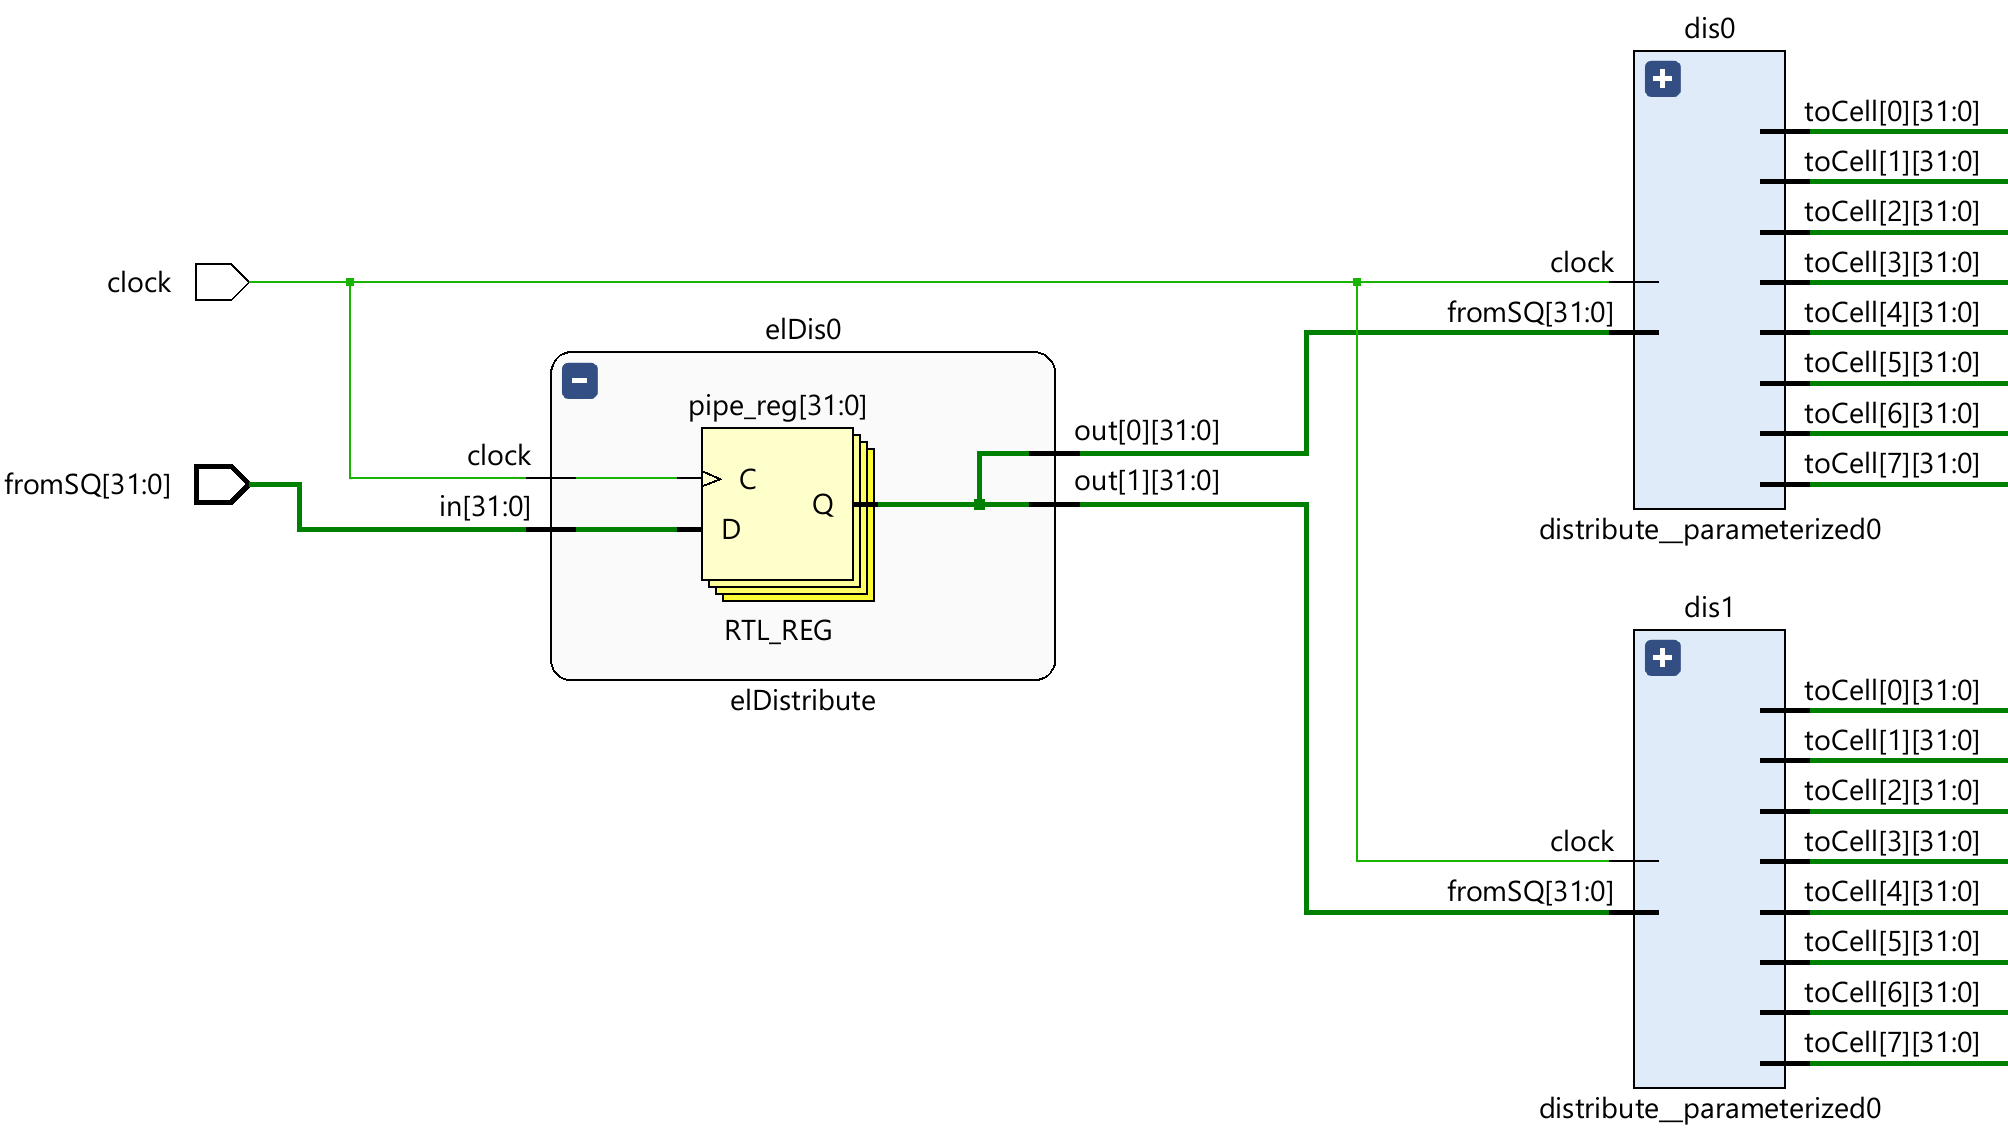
\includegraphics[width=\textwidth]{Images/distribute.png} 
    \caption{The recursively defined distribution network for $p=16$.}
    \label{fig:distribute}
\end{figure}
$\diamond$

\includeverilogcode[caption={Elementary distribution module.  File: elDistribute.sv. }, 
                    label={lst:elDistribute}, 
                    firstline=1, 
                    firstnumber=1, 
                    lastline=68]
                    {\verilogSourceDir/A14_elDistribute.sv}


\begin{problem}
Design for $p$ and simulate for $p=16$ the reduce network represented in Figure \ref{reduceNet}.

$\diamond$
\end{problem}

\begin{problem}\label{prob:scan}
Let us consider a $p$-input scan network with cells defined on two 34-bit inputs, {\tt in1} and {\tt in2}, and two 34-bit outputs, {\tt out1} and {\tt out2}, synchronized by the clock signal. Design a $p$-input scan network and implement it for $p=16$ in a version independent of the actual content of the cells, i.e., consider only the top level of the design. The pattern of a scan network is exemplified in Figure \ref{fig:scanRedTop} (ignore the output {\tt reduceOut}).

$\diamond$
\end{problem}

\begin{problem}
Redesign the scan network from Problem \ref{prob:scan} emphasizing the reduction output, {\tt reduceOut}, as in representation from Figure \ref{fig:scanRedTop}.

$\diamond$
\end{problem}